\documentclass[a4paper,10pt,french]{article}
\newcounter{question}%[section]
\newcounter{subquestion}%[section]
\newcommand{\question}{%
  \setcounter{subquestion}{0}
  \refstepcounter{question}%
  \paragraph{Question \thequestion}%
}

% Préambule; packages qui peuvent être utiles
   \RequirePackage[T1]{fontenc}        %
   \RequirePackage{babel,indentfirst}  % Pour les césures correctes,
                                       % et pour indenter au début de chaque paragraphe
   \RequirePackage[utf8]{inputenc}   % Pour pouvoir utiliser directement les accents
                                     % et autres caractères français
   \RequirePackage{lmodern,tgpagella} % Police de caractères
   \textwidth 17cm \textheight 25cm \oddsidemargin -0.24cm % Définition taille de la page
   \evensidemargin -1.24cm \topskip 0cm \headheight -1.5cm % Définition des marges
   \RequirePackage{latexsym}                  % Symboles
   \RequirePackage{amsmath}                   % Symboles mathématiques
   \RequirePackage{tikz}   % Pour faire des schémas
   \RequirePackage{graphicx} % Pour inclure des images
   \RequirePackage{listings} % pour mettre des listings
   \usetikzlibrary{shapes.geometric,positioning}
    
% Fin Préambule; package qui peuvent être utiles

\title{Rapport de TP 4MMAOD : Patch optimal entre deux fichiers}
\author{
	BOYER Quentin (groupe étudiant$_1$)
}

\begin{document}

\maketitle

\section{Graphe de dépendances (1 point)}
\begin{center}
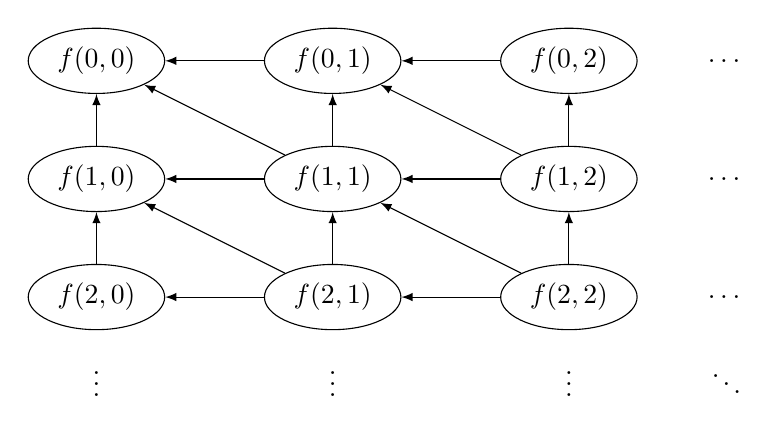
\begin{tikzpicture}
    \begin{scope}
		\node[ellipse, draw](0) at (0,0) {$f(0,0)$};
		\node[ellipse, draw](1) at (0,-1.5) {$f(1,0)$};
		\node[ellipse, draw](2) at (0,-3) {$f(2,0)$};

		\node[ellipse, draw](3) at (3,0) {$f(0,1)$};
		\node[ellipse, draw](4) at (3,-1.5) {$f(1,1)$};
		\node[ellipse, draw](5) at (3,-3) {$f(2,1)$};

		\node[ellipse, draw](6) at (6,0) {$f(0,2)$};
		\node[ellipse, draw](7) at (6,-1.5) {$f(1,2)$};
		\node[ellipse, draw](8) at (6,-3) {$f(2,2)$};

		\draw[-latex] (8) -- (5);
		\draw[-latex] (5) -- (2);

		\draw[-latex] (7) -- (4);
		\draw[-latex] (4) -- (1);

		\draw[-latex] (6) -- (3);
		\draw[-latex] (3) -- (0);

		\draw[-latex] (1) -- (0);
		\draw[-latex] (2) -- (1);

		\draw[-latex] (5) -- (4);
		\draw[-latex] (4) -- (3);

		\draw[-latex] (8) -- (7);
		\draw[-latex] (7) -- (6);

		\draw[-latex] (4) -- (0);
		\draw[-latex] (8) -- (4);
		\draw[-latex] (5) -- (1);
		\draw[-latex] (7) -- (3);

		\node at (0, -4) {\vdots};
		\node at (3, -4) {\vdots};
		\node at (6, -4) {\vdots};

		\node at (8, 0) {\ldots};
		\node at (8, -1.5) {\ldots};
		\node at (8, -3) {\ldots};

		\node at (8, -4) {$\ddots$};
	\end{scope}
\end{tikzpicture}
\end{center}

{L'algorithme est alors de trouver le plus court chemin depuis un point $(i,j) tq i=0 et/ou j=0$. Cela donne donc en fonction du chemin le patch optimal}

%%%%%%%%%%%%%%%%%%%%%%%%%%%%%%%%%%%%%%%%%%%%%%
\section{Principe de notre  programme (1 point)}
{
	Pour pouvoir trouver le plus court chemin je commence par creer une liste de tout les chemins au depart d'un des bords avec $i=0$ ou $j=0$. Ensuite on fait un tas avec ces chemins. A chaque iteration suivante on prends le chemin le plus court, on l'enleve du tas. Grace a ce chemin on produit trois chemin en incrementant $i$, $j$ puis $i$ et $j$.
	Si un chemin $c1$ arrive sur une case sur laquelle un autre chemin est deja passe, on sait par notre invariant qu'il existe un autre moyen d'arriver a ce point, et qu'il est plus court. On peut donc supprimer $c1$, puisque il sera pire que le chemin qui est deja passe par la.
	Sinon on ajoute le chemin dans notre tas

	On s'arrete des que le plus court chemin arrive sur la case $(m,n)$. On a alors trouve le plus court chemin pour arriver au patch optimal
	
	De plus pour calculer les couts on stock non pas un tableau des lignes mais un tableau qui donne l'indice de la fin de la ligne $i$, cela permet ainsi d'avoir un cout faible pour trouver la longeure d'une ligne
}

%%%%%%%%%%%%%%%%%%%%%%%%%%%%%%%%%%%%%%%%%%%%%%
\section{Analyse du coût théorique (3 points)}
%{\em Donner ici l'analyse du coût théorique de votre programme en fonction des nombres $n_1$ et $n_2$ de lignes
%et $c_1$ et $c_2$ de caractères des deux fichiers en entrée.
%Pour chaque coût, donner la formule qui le caractérise (en justifiant brièvement pourquoi cette formule correspond à votre programme),
%puis l'ordre du coût en fonction de $n_1, n_2, c_1, c_2$ en notation $\Theta$ de préférence, sinon $O$.}
{
	On commence par calculer la liste des indices de fin de ligne, ca coute $m+n$ dans tout les cas.
}

  \subsection{Nombre  d'opérations en pire cas\,: }
    \paragraph{Justification\,: }
	Dans le pire cas il faut calculer tout les chemins possibles, c'est a dire passer par chaque case exactement une fois, cela fait donc $m\times n$ iterations. A chaque iteration on produit environ 1 chemin, puisque si rentre en collision avec les autres chemins, au total on est donc en $\Theta(m\times n)$
  \subsection{Place mémoire requise\,: }
    \paragraph{Justification\,: }
	Dans chaque case on doit stocker de quelle cases viens t'on, pour pouvoir refaire le chemin dans le sens inverse. Cela fait donc dans le pire cas autant de place requise que de chemins, soit $\Theta(m\times n)$.
  \subsection{Nombre de défauts de cache sur le modèle CO\,: }
    \paragraph{Justification\,: }
	Pour les defauts de cache, dans le pire cas a chaque fois qu'on essaye d'acceder a une case elle n'est pas dans le cache, si par exemple les chemins les plus courts sont dans des parties totalement differentes de la grille. Cela coute donc $\Theta(m\times n)$

	\subsection{Quand arrive le pire cas}
{
	Si les fichiers ne sont pas tres differents on va rester majoritairement autour de la diagonale. Cela change donc beacoup la donne, puisque on va faire des defauts de cache que lorsque on a trop avance dans la diagonale, on va calculer et garder en memoire qu'environ la diagonale.

	Si $m\approx n$ on a la diagonale de longeure $m$, cela donne donc un algorithme quasiment lineaire en la taille des fichiers, et $m/L$ defauts de cache environ
}


%%%%%%%%%%%%%%%%%%%%%%%%%%%%%%%%%%%%%%%%%%%%%%
\section{Compte rendu d'expérimentation (2 points)}
  \subsection{Conditions expérimentaless}

    \subsubsection{Description synthétique de la machine\,:}
	Le CPU de la machine est un AMD Ryzen 2600, avec 16GB de RAM DDR4. Il tourne sur Arch Linux, i3. Utilisation standard du PC avec des logiciels usuels d'ouvert comme un navigateur web.

    \subsubsection{Méthode utilisée pour les mesures de temps\,: }
	J'ai utilise le benchTester pour relever les temps de chaque benchmark, user puisque c'est un programme mono-thread et que cela enleve le temps de l'OS. l'un apres l'autre en attendant. J'ai recommence 5 fois.

  \subsection{Mesures expérimentales}

    \begin{figure}[h]
      \begin{center}
        \begin{tabular}{|l||r||r|r|r||}
          \hline
          \hline
            & coût         & temps     & temps   & temps \\
            & du patch     & min       & max     & moyen \\
          \hline
          \hline
		  benchmark\_00 &   10354   &  0.03 &  0.06   &  0.04   \\
          \hline
		  benchmark\_01 &   12437   &  6.92 &  7.32   &  7.13   \\
          \hline
		  benchmark\_02 &   3559    &  5.24 &  5.64   &  5.42   \\
          \hline
		  benchmark\_03 &   19088   & 10.37 & 11.23   &  10.85  \\
          \hline
		  benchmark\_04 &   3707    &  4.16 &  4.34   &  4.25   \\
          \hline
          \hline
        \end{tabular}
        \caption{Mesures des temps minimum, maximum et moyen de 5 exécutions pour les benchmarks.}
        \label{table-temps}
      \end{center}
    \end{figure}

	On voit en annexe un graphe de temps de calcul en fonction de la taille de fichier, avec des fichiers qui different avec environ 30\% de probabilite par ligne

\subsection{Analyse des résultats expérimentaux}
On voit avec le graphe en annexe que le temps semble en effet etre entre quadratique et lineaire.

\section{Coût du patch en octet (1 point)}
Il suffit juste de changer la fonction de cout en disant que cela coute aussi cher de supprimer que d'ajouter, et quasmient deux fois plus cher de faire une subsititution. Le cout est alors approximativement la longeure de la ligne somme avec le nombre de chiffres pour representer le numero de la ligne. Cela change peu le probleme.
%%%%%%%%%%%%%%%%%%%%%%%%%%%%%%%%%%%%%%%%%%%%%%
\section{Bonus : Pourrait-on utiliser une technique de blocking ? (1 point)}
Avec l'algorithme tel que presente non, en effet on risque de ne pas trouver le chemin optimal puisque l'algorithme ne sait que aller dans le coin d'un bloc. Pour faire du blocking ca serait de couper les fichiers en parties de plus en plus petites et essayer de transformer chacune des parties d'entree en chacune des parties d'entrees. Le cout de recoller chaque partie risque de s'averer assez haut

\section*{Annexe}

    \begin{figure}[h]
      \begin{center}
		  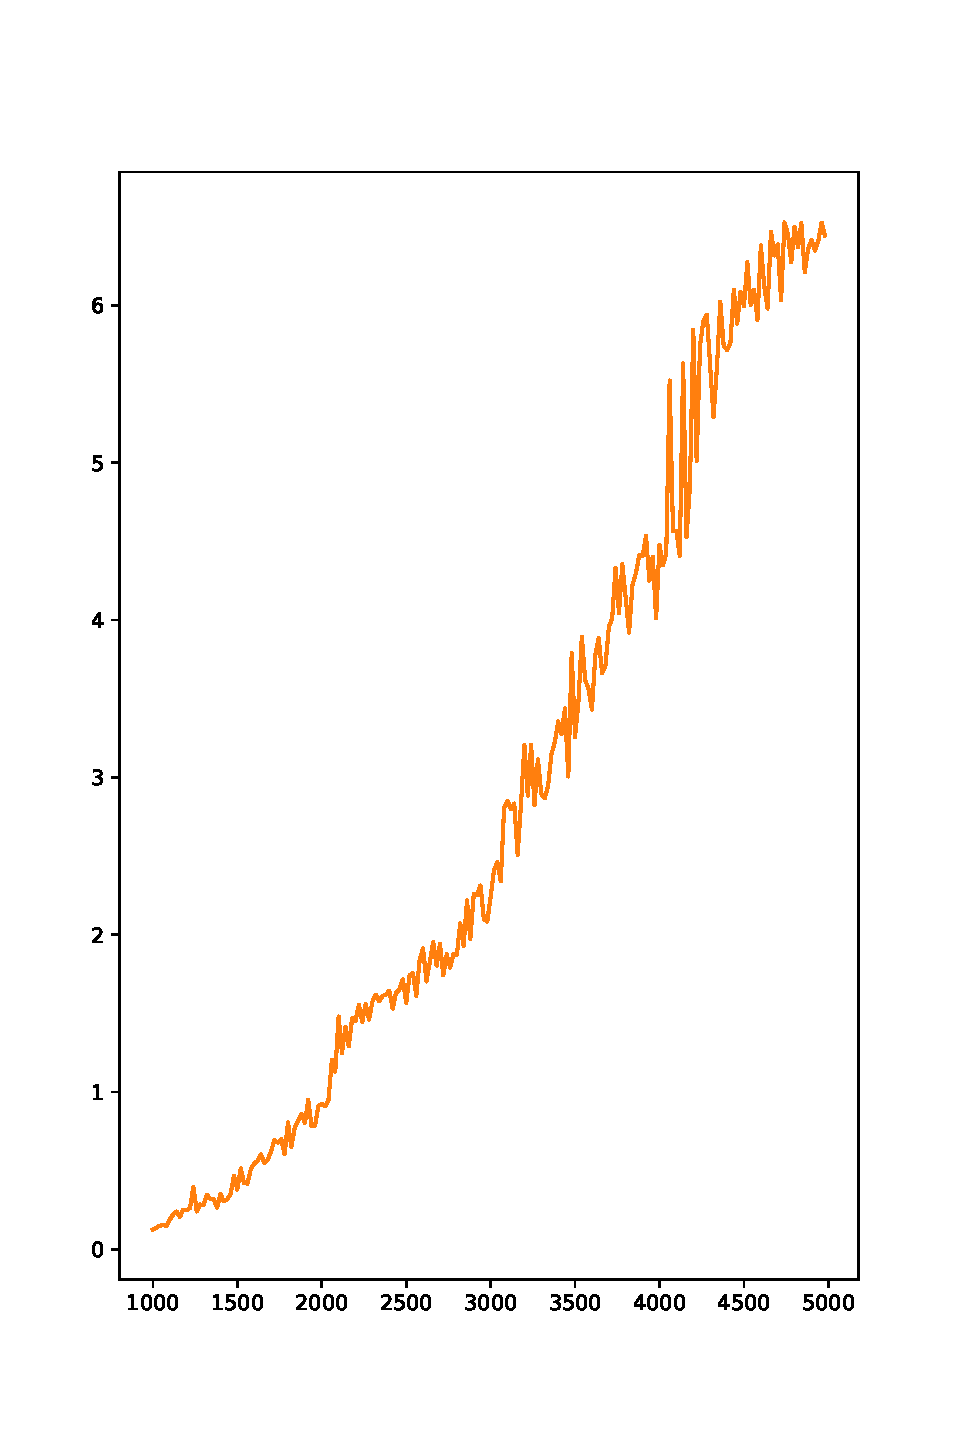
\includegraphics{rapport/cost.pdf}
		  \caption{Mesures des temps minimum en fonction de la longeure}
		  \label{graph-temps}
      \end{center}
    \end{figure}

\end{document}
%% Fin mise au format
